\xiti
\begin{xiaotis}
\begin{enhancedline}

\xiaoti{从一个正方体中,如图那样截去四个三棱锥后,得到一个正三棱锥 $A{-}BCD$,求它的体积是正方体体积的几分之几?}

\begin{figure}[htbp]
    \centering
    \begin{minipage}[b]{7cm}
        \centering
        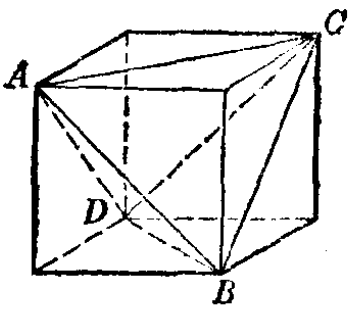
\includegraphics[width=5cm]{../pic/ltjh-ch2-xiti13-01.png}
        \caption*{(第 1 题)}
    \end{minipage}
    \qquad
    \begin{minipage}[b]{7cm}
        \centering
        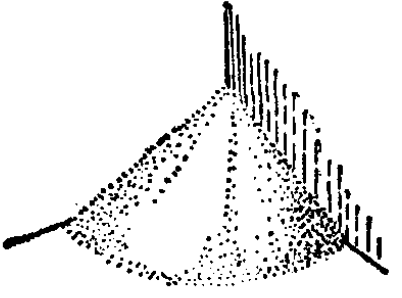
\includegraphics[width=5cm]{../pic/ltjh-ch2-xiti13-04.png}
        \caption*{(第 4 题)}
    \end{minipage}
\end{figure}

\xiaoti{在下列情形下,正棱锥的体积有什么变化:}
\begin{xiaoxiaotis}

    \xxt{高和底面的边长都增为原来的 $n$ 倍;}

    \xxt{高增为原来的 $n$ 倍,底面边长缩为原来的 $\exdfrac{1}{n}$。}

\end{xiaoxiaotis}


\xiaoti{已知下列各正棱锥的底面边长是 $a$,侧棱长是 $b$。求它的体积:
    (1)正三棱锥;(2)正四棱锥;(3)正六棱锥。
}

\xiaoti{在仓库一角有谷一堆,呈 $\exdfrac{1}{4}$ 圆锥形(如图)。量得底面弧长为 2.8 m,
    母线长为 2.2 m。这堆谷重约多少(谷的比重:$720\;\qkmlfm$)?
}

\xiaoti{有一铜制工件,它的下部呈正四棱柱形,顶部是一个以正四棱柱的上底为底的正四棱锥形。
    柱的底面边长是 50 mm,高是 40 mm,锥的侧面呈正三角形。
    求这个工件的重量(钢的比重是 $8.9\;\kmlflm$)。
}

\xiaoti{三棱锥的三个侧面互相垂直,它们的面积分别为 $6\;\pfm$、$4\;\pfm$ 和 $3\;\pfm$。求它的体积。}

\xiaoti{从一块薄铁板上,裁下一个半径为 24 cm,圆心角为 $120^\circ$的扇形,再围成一个圆锥筒。
    求这个圆锥筒的容积(保留两位有效数字)。
}

\xiaoti{圆锥的体积是 $22.4\;\lflm$,轴和母线所成的角是 $48^\circ15'$。求它的高(保留三位有效数字)。}

\xiaoti{求证:棱锥被平行于底面的平面截得的小棱锥的体积和原来棱锥的体积的比,等于它们的高的立方比。}

\end{enhancedline}
\end{xiaotis}

